% =====================================================================
%  Capítulo 6 — Cuestiones legales
% =====================================================================
\chapter{Cuestiones legales}

Toda agresión puede tener dos tipos principales de consecuencias:

\begin{enumerate}
  \item \textbf{Físicas:} en la salud de la víctima o del agresor (heridas o muerte). Con frecuencia la víctima puede quedar con secuelas psicológicas de largo tratamiento, aun sin sufrir daño físico.
  \item \textbf{Legales:} dado que no pretendemos atacar a nadie, cualquier violencia ejercida sobre quien nos agrede parecería justificada. Sin embargo, para la ley esto no es tan sencillo.
\end{enumerate}

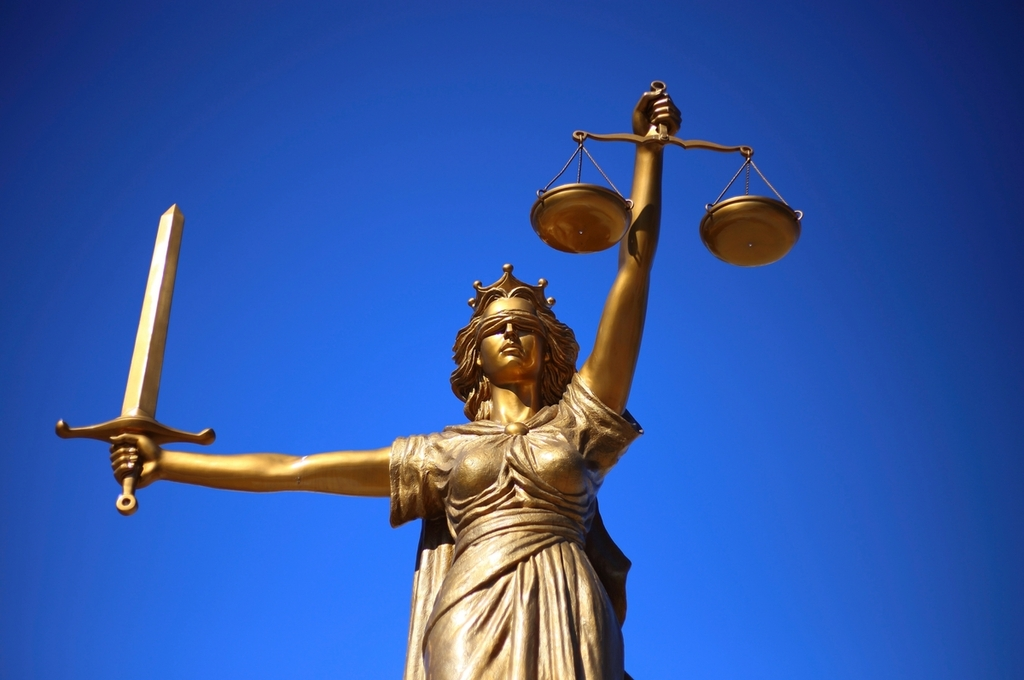
\includegraphics[width=\linewidth]{figures/ley.jpg}

\section{La legítima defensa en España (art.\ 20.4 del Código Penal)}

El Código Penal español \citep{codigopenal1995} exime de responsabilidad criminal a quien obra en defensa de la persona o derechos propios o ajenos, siempre que concurran tres requisitos:

\begin{enumerate}
  \item \textbf{Agresión ilegítima:} un ataque actual o inminente contra ti, otra persona o tus bienes. No vale frente a una agresión ya terminada (entonces sería represalia).
  \item \textbf{Necesidad racional del medio empleado:} la respuesta debe ser razonable para impedir o repeler la agresión, valorando las circunstancias (tamaño y número de agresores, armas, lugar, hora, posibilidad real de huir). No se exige una igualdad matemática de medios: la jurisprudencia reconoce que una mujer frente a un agresor físicamente superior puede necesitar medios más contundentes para defenderse con eficacia.
  \item \textbf{Falta de provocación suficiente:} que quien se defiende no haya provocado la agresión.
\end{enumerate}

El concepto de \enquote{arma} no está reservado a las de fuego y blancas: es todo elemento que aumenta el poder ofensivo de una persona y puede ocasionar lesiones o la muerte. Ten en cuenta, además, que en España está prohibido portar armas e imitaciones en la vía pública (Reglamento de Armas), y que los esprays de defensa solo son legales los homologados por Sanidad para mayores de edad.

Se deben tener en cuenta también las circunstancias: no es lo mismo defenderse de noche de un ladrón que, en pleno día, de un individuo con sus sentidos alterados por alguna droga; la justicia puede valorar su estado, y si causamos daños deberemos poder acreditar que no había otra posibilidad (testigos, cámaras, etc.).

\textbf{Nuestro consejo práctico:} lo primero es salir de la situación de peligro; de las consecuencias nos preocuparemos después. No sabemos cuáles son las intenciones del agresor, así que lo mejor es librarse de él cuanto antes. Solucionemos los problemas según nos vamos encontrando con ellos. La mejor salida de un enfrentamiento sigue siendo evitar el uso de la fuerza, por sus posibles consecuencias: daños físicos o psicológicos, problemas judiciales y posibles venganzas. Y recuerda: no merece la pena sufrir daños por defender un bien material.

\section{Después de una agresión}

\begin{itemize}
  \item Ponte a salvo y llama al \recurso{112} (emergencias) o usa el botón SOS de AlertCops.
  \item Si has sufrido una agresión sexual, acude a urgencias hospitalarias sin lavarte ni cambiarte de ropa, para preservar pruebas; allí se activa el protocolo forense y de atención.
  \item Denuncia en Policía Nacional (\recurso{091}), Guardia Civil (\recurso{062}) o juzgado de guardia. Aporta todos los datos que hayas podido registrar: lugar, número de agresores, edades, armas, estatura, ropa, tatuajes y particularidades.
  \item Las Oficinas de Asistencia a las Víctimas del Delito (Ministerio de Justicia) ofrecen apoyo jurídico y psicológico gratuito.
\end{itemize}

Este capítulo es divulgativo y no constituye asesoramiento jurídico; ante un caso concreto consulta con un abogado.
